\chapter{Evaluation} % (fold)
\label{cha:evaluation}

\section{Evaluation Methodology} % (fold)
\label{sec:evaluation:evaluation_methodology}

This chapter present the results of each technique described on Chapter \ref{cha:tracking_library_for_the_web}. Two metrics were utilized to analyze the solutions available on \textit{tracking.js} library:

\begin{enumerate}
	\item Performance: frames per second (FPS) metric of how the implemented techniques performs on the web environment in order to reach real-time capability. On the United Kingdom popular video format known as Phase Alternating Line (PAL) \cite{PAL1962}, real time video is represented by 25 FPS, therefore this value is used to define whether the tests can or cannot be considered real-time. The FPS metric were extracted from the frames rendered in the last second for the canvas element being tested only, that way only the important data were being computed in order to not affect the result numbers. Browsers have intrinsic performance limitations (Section \ref{sec:basic_concepts:web}), utilizing performance as a metric is important in order to proof that tracking techniques could be a reality on the web environment. All performance tests were run inside the web browser. The browser JavaScript code interpretation latency is computed in the numbers presented, thus respecting the real usage performance running from the web environment.
	\item Partial occlusion robustness: present tests how the implemented techniques reacts to partial occlusions. The web users are usually novice, from those users, requiring some training or calibration before using tracking solutions is overwhelming. The web users can potentially have unexpected behaviors when using a tracking application in front of a computer, and partial occlusion is one of them. Therefore the importance of measuring random partial occlusions on web techniques is to understand how the implementation reacts to that situations. This work considered robust to a partial occlusion situations that the tracked object was still able to be identified with the addition of random occlusions caused by the user fingers.
\end{enumerate}

Several tracking techniques are already available in server-side languages, such as C/C++, OpenCV \cite{Bradski2000} is an example of a library with those capabilities. Integrating existing libraries in tracking solutions on the web was, at first glance, much doable, since the code base was already available, on the other hand the web browsers are not able to run C/C++ directly. In order to run those existing technologies, several approached were tested on \cite{Pablo2013}: using client to server requests in order to process video frames; or trough platform dependent plugins, such as OSAKit \cite{OSAKit2013}, that allowed OpenCV library to run on the client-side \cite{Pablo2013}. A comparison between \textit{tracking.js} and those existing solutions involving client and server-side tracking is discussed on subsection \ref{sec:evaluation:js_tracking_solution}, showing some benefits of a pure JavaScript client-side tracking solution.

Google Chrome browser is the current most popular web browser, for that reason, all tests were executed on Google Chrome browser version 28.0.1500.71 \cite{Chrome2010}, running on Mac OS X 10.8.3, 2.6 GHz Intel Core i7 16 GB 1600 MHz RAM.

% section evaluation_methodology (end)

\section{Rapid Object Detection (Viola Jones)} % (fold)
\label{sec:evaluation:results:rapid_object_detection}

\subsection{Description} % (fold)
\label{sub:evaluation:rapid_object_detection:description}

Having Viola Jones rapid object detection as part of the library resulted in interesting examples for web applications, such as detecting faces, mouths, eyes and any other training data \cite{Viola2001}. All training data tested were imported from OpenCV \cite{Bradski2000} and converted to JSON \cite{Crockford2013}. On Figure \ref{figure:viola_overview} is shown different examples of training data being used by the library implementation of Viola Jones.

\begin{figure}[!htb]
  \centering
  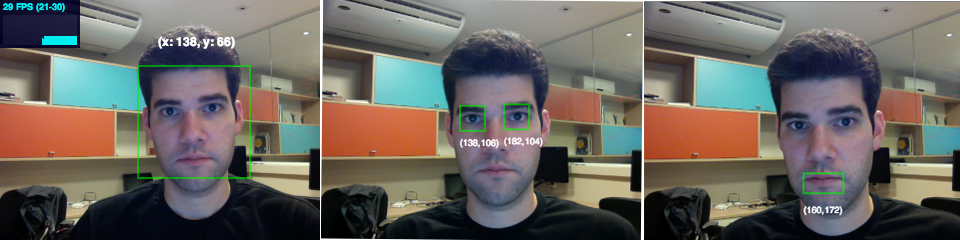
\includegraphics[width=\linewidth]{chapters/evaluation/viola_overview.png}
  \caption{Library implementation of Viola Jones using different training datas for detecting faces, eyes and mouth.}
  \label{figure:viola_overview}
\end{figure}

\begin{figure}[!htb]
  \centering
  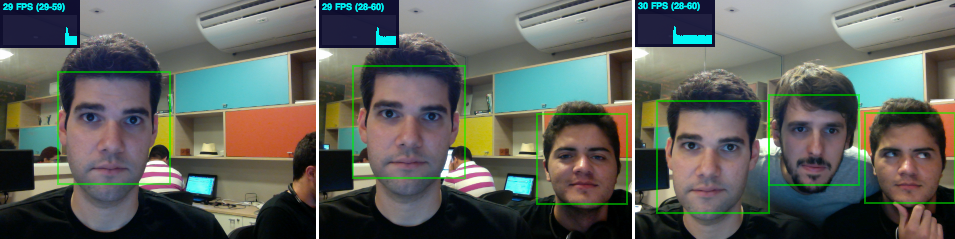
\includegraphics[width=\linewidth]{chapters/evaluation/viola.png}
  \caption{Library implementation of Viola Jones detecting multiple faces inside the real-time limit of 25 FPS.}
  \label{figure:viola_multiple_faces}
\end{figure}

Augmented reality and tracking applications for advertising and entertainment are gaining more space on the web enviroment. The media used in this kind of application needs to be as appealing as possible in order to catch consumers' attention, thus detecting faces, or augmenting the scene with objects are attractive possibilities. In order to demonstrate that concept, a simple chat application was created. In this chat application, while talking in real-time, the users could augment their faces with objects, such as a fake glass with mustache. In order to extract the users face coordinates Viola Jones was used. Listing \ref{lst:viola} shows the simplified JavaScript API provided by \textit{tracking.js} in order to extract face coordinates and draw the image. The fake glasses are positioned over $x$ and $y$ coordinates on the canvas axis based on the extracted values. Figure \ref{figure:viola_glass_face} demonstrates the described example.

\begin{figure}[!htb]
  \centering
  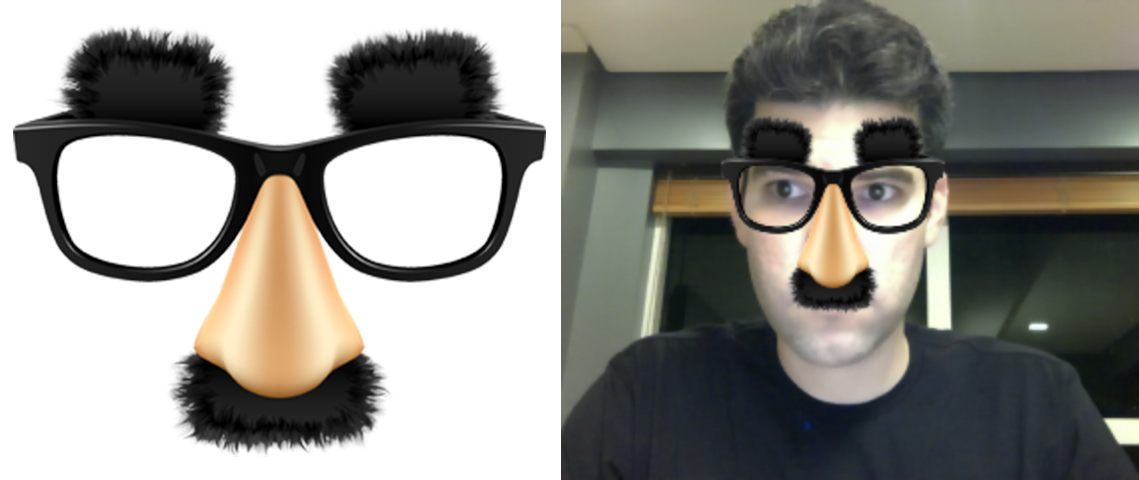
\includegraphics[width=380pt]{chapters/evaluation/viola_glass_face.png}
  \caption{Augmenting users faces with objects using \textit{tracking.js} Viola Jones eyes detection.}
  \label{figure:viola_glass_face}
\end{figure}

\begin{lstlisting}[language=C++,label={lst:viola},caption=Example of \textit{tracking.js} API of augmenting users faces with objects using Viola Jones face detection.]
  var img = new Image();
  img.src = 'img/glasses.png';
  var videoCamera = new tracking.VideoCamera();
  videoCamera.track({
      type: 'human',
      data: 'frontal_face',
      onFound: function(track) {
          videoCamera.canvas.context.drawImage(img, track[0].x, track[0].y, track[0].size, track[0].size);
      }
  });
\end{lstlisting}

% subsection description (end)

\subsection{Results} % (fold)
\label{sub:evaluation:rapid_object_detection:results}

\subsubsection{Performance} % (fold)
\label{subsub:evaluation:rapid_object_detection:results:performance}

The United Kingdom popular video format known as Phase Alternating Line (PAL) \cite{PAL1962} defines that real time video is represented by 25 FPS, therefore this value is used to define whether the tests can or cannot be considered real-time. On Figure \ref{figure:viola_fps}, the Viola Jones implementation were tested with different numbers of detected faces. Fifteen faces were gradually added, for each addition the FPS average was recorded. Note that, until five faces detected the web implementation still runs inside the real-time limit defined by PAL \cite{PAL1962}.

\begin{figure}[!htb]
  \centering
    \begin{tikzpicture}
    \begin{axis}[
        enlarge x limits=0.03,
        minor tick num=1,
        xlabel=Number of detected faces,
        ylabel=Frames per second (FPS)]

        \addplot[wblue,mark=x] coordinates {
             (1,30)
             (2,29)
             (3,30)
             (4,27)
             (5,25)
             (6,20)
             (7,17)
             (8,16)
             (9,16)
             (10,15)
             (11,15)
             (12,13)
             (13,11)
             (14,9)
             (15,8)
         };

         \draw [red] ({rel axis cs:0,0}|-{axis cs:15,25}) -- ({rel axis cs:1,0}|-{axis cs:15,25}) node [pos=0.0, above] {};
    \end{axis}
    \end{tikzpicture}
   \caption{Library implementation of Viola Jones tested with different numbers of detected faces.}
   \label{figure:viola_fps}
\end{figure}

% subsubsection performance (end)

\subsubsection{Oclusion Robustness} % (fold)
\label{subsub:evaluation:rapid_object_detection:results:occlusion_robustness}

Viola Jones implementation of \textit{tracking.js} is robust for random partial occlusions. Figure \ref{figure:viola_occlusion} demonstrates occlusions variations that still allows the face to be detected.

\begin{figure}[!htb]
  \centering
  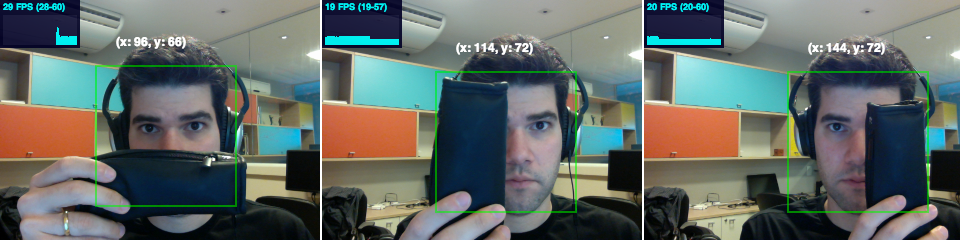
\includegraphics[width=\linewidth]{chapters/evaluation/viola_occlusion.png}
  \caption{Library implementation of Viola Jones partial occlusion robustness.}
  \label{figure:viola_occlusion}
\end{figure}

% subsubsection occlusion_robustness (end)

\subsection{Discussion} % (fold)
\label{sub:evaluation:rapid_object_detection:discussion}

The this section shows rapid object detection as an interesting technique to be available on \textit{tracking.js}. It provides ways to detect user faces, eyes and any other training data available, resulting in attractive tracking and AR solutions on the web. Future work is required in order to leverage this technique to be robust enough in order to be used in real large applications. The first improvement that could be done is on performance. The average result performance is inside the real-time limit defined by PAL \cite{PAL1962}, although an optimization on the training JSON data structure can be still made in order to avoid nested arrays, where each array contains float numbers. That optimization allows the usage of typed float arrays to store the training numbers, resulting in a overall FPS speed improvement of $30\%$. The second improvement is apply a Double Exponential Smoothing technique to the detection. It's an Alternative to Kalman Filter-Based Predictive Tracking \cite{LaViola2003}. Predictive tracking algorithms represent an important component of any tracking or AR system. Without these algorithms, tracking and AR systems must use image processing or pose calculation for each frame. This naive approach can cause problems, such as display-to-user-motion synchronization mismatch. This mismatch degrades the user experience because dynamic tracking error produces perceived latency and possible cybersickness \cite{LaViolaJr.2000}.

% subsection discussion (end)

% section rapid_object_detection (end)

\section{Color Tracking Algorithm} % (fold)
\label{sec:evaluation:color_tracking_algorithm}

\subsection{Description} % (fold)
\label{sub:evaluation:results:color_tracking_algorithm:description}

Being able to use colored objects to control your browser using the user camera is very appealing. Any colored object could be used to enable user interaction with your web application using \textit{tracking.js} color tracking technique trough a simple and intuitive JavaScript API (Listing \ref{lst:color}). On Figure \ref{figure:color_object} is shown different colored objects being tracked.

\begin{figure}[!htb]
  \centering
  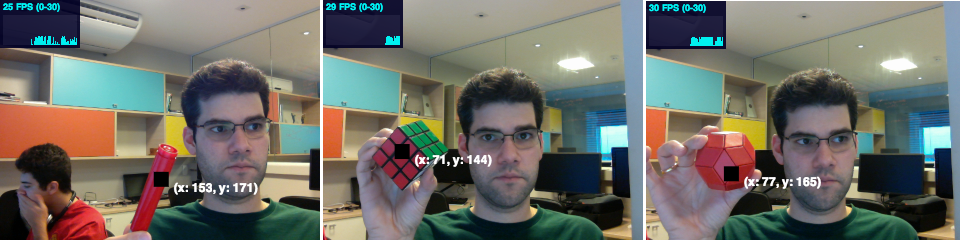
\includegraphics[width=\linewidth]{chapters/evaluation/color_object.png}
  \caption{Library implementation of color tracking for different objects: On the left a red pencil marker; on the center a Rubik's magic cube \cite{Rubiks2013} from the red face; and on the right a red Ball of Whacks \cite{Whack2013}.}
  \label{figure:color_object}
\end{figure}

\begin{lstlisting}[language=C++,label={lst:color},caption=Example of \textit{tracking.js} color API.]
  var videoCamera = new tracking.VideoCamera();
  videoCamera.track({
      type: 'color',
      color: 'magenta',
      onFound: function(track) {
        // do your logic here.
      }
  });
\end{lstlisting}

Enable entertainment web applications is also possible using color tracking. Few examples were implemented using color tracking and a PlayStation move controller (Figure \ref{figure:psmove}) that is basically a colored sphere that can emit light, the color of the sphere can be set via Bluetooth. This controller have four buttons, square, triangle, cross, circle, which are color coded as pink, green, blue and red. The controller has also three types of built-in sensors, temperature, accelerometer, gyroscope and magnetometer. In this work only the emitted light is used to track the scene.

\begin{figure}[!htb]
  \centering
  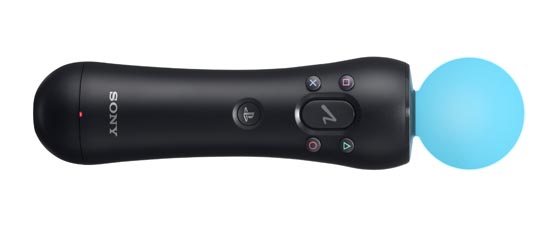
\includegraphics[width=280pt]{chapters/evaluation/psmove.png}
  \caption{PlayStation move controller.}
  \label{figure:psmove}
\end{figure}

On Figure \ref{figure:color_games}, the two bottom images are examples of how games could be developed to the web trough color tracking. On the bottom left, a multi-player game that allows the user to draw in order to competitors guess what is the drawing meaning is demonstrated. On the bottom right, multiple PlayStation move controllers are used to control the user interactions into a 3D environment rendered trough the GPU using WebGL \cite{WebGL2013}. Note that, the available \textit{tracking.js} techniques could be combined with WebGL rendering in order to reach real-time 3D rendering.

\begin{figure}[!htb]
  \centering
  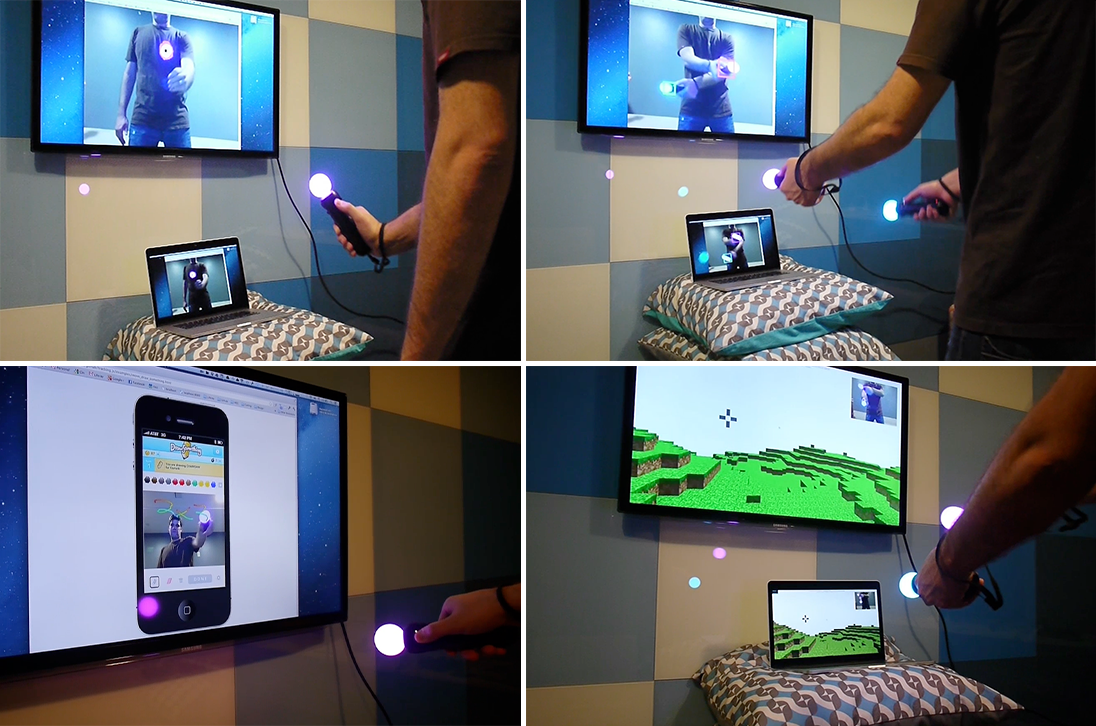
\includegraphics[width=\linewidth]{chapters/evaluation/color_games.png}
  \caption{Library implementation of color tracking used in games running on the web. On the Bottom left, a multi-player game that allows the user to draw using the camera. On the bottom right, multiple PlayStation move controllers are used to control the user interactions into a 3D environment.}
  \label{figure:color_games}
\end{figure}

Another example of color tracking on user interactions is demonstrated on Figure \ref{figure:color_volume}. Using a HTML5 audio element \cite{International2009} a music is played and trough any colored object, the user can control the volume of the player sliding the object from the left to right and vice-versa, left most coordinates means volume set to zero, right most coordinates means volume set to maximum.

\begin{figure}[!htb]
  \centering
  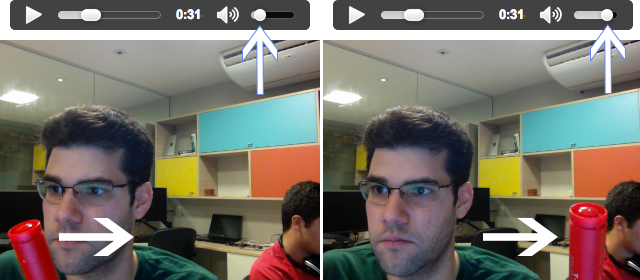
\includegraphics[width=\linewidth]{chapters/evaluation/color_volume.png}
  \caption{Library implementation of color tracking controlling the HTML5 audio element volume.}
  \label{figure:color_volume}
\end{figure}

% subsection description (end)

\subsection{Results} % (fold)
\label{sub:evaluation:color_tracking_algorithm:results}

\subsubsection{Performance} % (fold)
\label{subsub:evaluation:color_tracking_algorithm:results:performance}

On Figure \ref{figure:color_fps}, the color tracking implementation were tested with different numbers of pixels detected. The size of the detect object were gradually increased, resulting in a bigger number of pixels found, for each incrementation in the size the FPS average was recorded. Note that, until $2138$ pixels detected the web implementation still runs inside the real-time limit defined by PAL \cite{PAL1962}.

\begin{figure}[!htb]
  \centering
    \begin{tikzpicture}
    \begin{axis}[
        enlarge x limits=0.03,
        minor tick num=1,
        xlabel=Number of pixels detected,
        ylabel=Frames per second (FPS)]

        \addplot[wblue,mark=x] coordinates {
        (174,30)
        (178,30)
        (178,30)
        (172,30)
        (164,30)
        (164,30)
        (150,30)
        (150,30)
        (156,30)
        (192,30)
        (192,30)
        (200,30)
        (200,30)
        (184,30)
        (160,30)
        (160,30)
        (160,30)
        (160,30)
        (158,30)
        (158,30)
        (162,30)
        (162,30)
        (180,30)
        (160,30)
        (160,30)
        (154,30)
        (154,30)
        (162,30)
        (162,30)
        (194,30)
        (194,29)
        (172,29)
        (172,29)
        (182,29)
        (134,29)
        (134,29)
        (160,29)
        (160,29)
        (176,29)
        (176,29)
        (154,29)
        (154,29)
        (184,29)
        (184,29)
        (172,29)
        (182,29)
        (182,29)
        (164,29)
        (164,29)
        (148,29)
        (148,29)
        (122,29)
        (122,29)
        (122,29)
        (138,29)
        (138,29)
        (162,29)
        (162,29)
        (176,29)
        (176,29)
        (208,30)
        (208,30)
        (208,30)
        (208,30)
        (200,30)
        (202,30)
        (202,30)
        (194,30)
        (194,30)
        (198,30)
        (198,30)
        (246,30)
        (246,30)
        (308,30)
        (308,30)
        (274,30)
        (254,30)
        (254,30)
        (322,30)
        (322,30)
        (406,30)
        (406,30)
        (434,30)
        (434,30)
        (408,30)
        (412,30)
        (470,30)
        (478,30)
        (478,30)
        (478,30)
        (546,29)
        (668,29)
        (668,29)
        (660,29)
        (700,29)
        (700,29)
        (756,29)
        (756,29)
        (848,29)
        (848,29)
        (890,29)
        (890,29)
        (884,29)
        (884,29)
        (880,29)
        (914,29)
        (914,29)
        (910,29)
        (910,29)
        (934,29)
        (934,29)
        (908,29)
        (908,29)
        (898,29)
        (974,29)
        (974,29)
        (998,29)
        (998,29)
        (1016,29)
        (1016,29)
        (1100,30)
        (1100,30)
        (1044,30)
        (1044,30)
        (1090,30)
        (1074,30)
        (1074,30)
        (1160,30)
        (1160,30)
        (1170,30)
        (1170,30)
        (1222,30)
        (1222,30)
        (1160,30)
        (1160,30)
        (1216,30)
        (1170,30)
        (1170,30)
        (1108,30)
        (1108,30)
        (1110,30)
        (1110,30)
        (1148,30)
        (1148,30)
        (1158,30)
        (1140,30)
        (1140,30)
        (1202,30)
        (1232,30)
        (1232,29)
        (1342,29)
        (1342,29)
        (1362,29)
        (1472,29)
        (1548,29)
        (1638,29)
        (1638,29)
        (1762,29)
        (1822,29)
        (1822,29)
        (1814,29)
        (1850,29)
        (1880,29)
        (1880,29)
        (1856,29)
        (1854,29)
        (1854,29)
        (1974,29)
        (1980,29)
        (1992,29)
        (2076,29)
        (2138,29)
        (2138,23)
        (2202,23)
        (2288,23)
        (2288,23)
        (2366,23)
        (2366,23)
        (2386,23)
        (2432,23)
        (2466,23)
        (2466,23)
        (2548,23)
        (2632,23)
        (2632,23)
        (2692,23)
        (2738,23)
        (2742,23)
        (2742,23)
        (2854,23)
        (2812,23)
        (2812,23)
        (2852,19)
        (2856,19)
        (2914,19)
        (2914,19)
        (2974,19)
        (2974,19)
        (2976,19)
        (3042,19)
        (3026,19)
        (3080,19)
        (3090,19)
        (3146,19)
        (3130,19)
        (3142,19)
        (3142,19)
        (3156,19)
        (3186,19)
        (3198,19)
        (3208,19)
        (3218,18)
        (3220,18)
        (3220,18)
        (3286,18)
        (3316,18)
        (3376,18)
        (3370,18)
        (3392,18)
        (3404,18)
        (3408,18)
        (3442,18)
        (3450,18)
        (3492,18)
        (3516,18)
        (3518,18)
        (3516,18)
        (3512,15)
        (3502,15)
        (3524,15)
        (3546,15)
        (3550,15)
        (3560,15)
        (3586,15)
        (3616,15)
        (3654,15)
        (3692,15)
        (3692,15)
        (3718,15)
        (3766,15)
        (3820,15)
        (3824,15)
        (3852,15)
        (3894,15)
        (3948,15)
        (3988,15)
        (4024,15)
        (4068,15)
        (4150,15)
        (4314,15)
        (4500,15)
        (4612,15)
        (4670,15)
        (4784,15)
        (4894,15)
        (4912,15)
        (4920,13)
        (4994,13)
        (5062,13)
        (5160,13)
        (5218,13)
        (5230,13)
        (5378,13)
        (5404,13)
        (5494,13)
        (5590,13)
        (5626,13)
        (5734,11)
        (5816,11)
        (5942,11)
        (6108,11)
        (6278,11)
        (6370,11)
        (6450,11)
        (6528,11)
        (6770,11)
        (6806,9)
        (7040,9)
        (7246,9)
        (7448,9)
        (7698,9)
        (7788,9)
        (7846,9)
        (7882,7)
        (7940,7)
        (7996,7)
        (8012,7)
        (7966,7)
        (7412,7)
         };

         \draw [red] ({rel axis cs:0,0}|-{axis cs:15,25}) -- ({rel axis cs:1,0}|-{axis cs:15,25}) node [pos=0.0, above] {};
    \end{axis}
    \end{tikzpicture}
   \caption{Library implementation of color tracking technique tested with different numbers of pixels detected.}
   \label{figure:color_fps}
\end{figure}

% subsubsection performance (end)

\subsubsection{Oclusion Robustness} % (fold)
\label{subsub:evaluation:color_tracking_algorithm:results:occlusion_robustness}

Color tracking technique implementation of \textit{tracking.js} is robust for random partial occlusions. Figure \ref{figure:color_occlusion} demonstrates occlusions variations that still allows the colored object to be detected.

\begin{figure}[!htb]
  \centering
  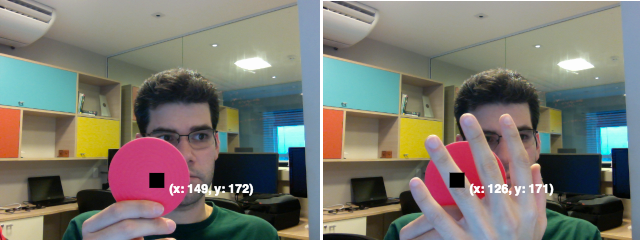
\includegraphics[width=\linewidth]{chapters/evaluation/color_occlusion.png}
  \caption{Library implementation of color tracking technique partial occlusion robustness.}
  \label{figure:color_occlusion}
\end{figure}

% subsubsection occlusion_robustness (end)

\subsection{Discussion} % (fold)
\label{sub:evaluation:color_tracking_algorithm:discussion}

The color tracking technique could use any colored object to control your web browser in an simple and fast way, the results seems to be very attractive. Future work is required in order to leverage this technique to be robust enough in order to be used in real large applications. An important improvement is to automatic calculate colors threshold. In the current implementation, the distance threshold value for each color was empirically defined, when drastic illumination changes happens the detection quality can be reduced since colors are directly affected by illumination variations. A threshold iteration test could be executed during the algorithm initialization in order to find the value that provides the highest number pixels from the set color.

% subsection discussion (end)

% section color_tracking_algorithm (end)

\section{Markerless Tracking Algorithm} % (fold)
\label{sec:evaluation:markerless_tracking_algorithm}

\subsection{Description} % (fold)
\label{sub:evaluation:markerless_tracking_algorithm:description}

Being able to track any object based on invariant natural features characteristics is also demonstrated by the markerless tracking technique. On Figure \ref{figure:keypoints_building} is shown features extracted from different scenes. Note that most part of the keypoints are invariant to the camera rotation. Based on the features detected, the best $H$ homography matrix is estimated. All found points in the first frame is multiplied by $H$ in order to be plotted in the second frame. The found $H$ is defined as follows:

$$H=\begin{pmatrix}1.6101363130102753 & -0.5346783206945362 & -33.21640286774384\\ 0.18027586959550446 & 0.8414271531603306 & -7.530803625100701\\ 0.0021658540103673164 & -0.0025444273054841503 & 1\\\end{pmatrix}.$$

\begin{figure}[!htb]
  \centering
  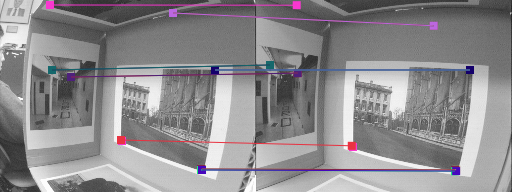
\includegraphics[width=\linewidth]{chapters/evaluation/keypoints_building.png}
  \caption{Library implementation of markerless tracking technique. Features are extracted from different scenes. On the first frame, $49$ features were detected by FAST \cite{RostenFaster2010}, on the second frame $17$ of those were matched by BRIEF \cite{Calonder2010} and plotted by the $H$ matrix.}
  \label{figure:keypoints_building}
\end{figure}

The markerless tracking web implementation have also showed to be robust for illumination and scaling differences. On Figure \ref{figure:keypoints_fast_brief} is shown the features detected by FAST (top images) and features extracted by BRIEF (bottom images) plotted based on the estimated homography $H$.

\begin{figure}[!htb]
  \centering
  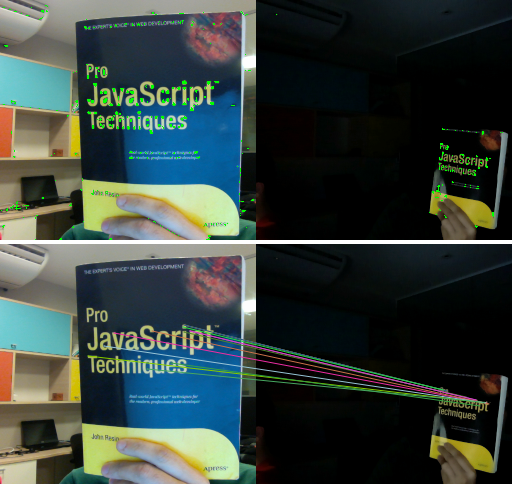
\includegraphics[width=\linewidth]{chapters/evaluation/keypoints_fast_brief.png}
  \caption{Library implementation of markerless tracking technique. Illumination and scaling robustness for features detected using FAST (top images) and extracted using BRIEF (bottom images) plotted on the second frame by the estimated homography matrix $H$.}
  \label{figure:keypoints_fast_brief}
\end{figure}

% subsection description (end)

\subsection{Results} % (fold)
\label{sub:evaluation:markerless_tracking_algorithm:results}

\subsubsection{Performance} % (fold)
\label{subsub:evaluation:markerless_tracking_algorithm:results:performance}

On Figure \ref{figure:markerless_fps}, the markerless tracking implementation were tested in an interval of $1000$ seconds. The FPS average for this technique is 6 FPS, which is not ideal for real-time applications yet. Some optimizations could be applied on future work, such as implementing FAST-ER \cite{RostenFaster2010} for feature detection.

\begin{figure}[!htb]
  \centering
    \begin{tikzpicture}
    \begin{axis}[
        enlarge x limits=0.03,
        minor tick num=1,
        xlabel=Time (seconds),
        ylabel=Frames]

        \addplot[wblue,mark=x] coordinates {
        (0,25)
        (5,5)
        (10,4)
        (15,4)
        (20,4)
        (25,5)
        (30,4)
        (35,5)
        (40,4)
        (45,5)
        (50,4)
        (55,4)
        (60,4)
        (65,4)
        (70,5)
        (75,5)
        (80,5)
        (85,5)
        (90,4)
        (95,5)
        (100,4)
        (105,5)
        (110,4)
        (115,4)
        (120,5)
        (125,4)
        (130,4)
        (135,4)
        (140,5)
        (145,5)
        (150,4)
        (155,5)
        (160,4)
        (165,5)
        (170,4)
        (175,5)
        (180,4)
        (185,5)
        (190,5)
        (195,4)
        (200,4)
        (205,5)
        (210,5)
        (215,4)
        (220,5)
        (225,5)
        (230,5)
        (235,4)
        (240,5)
        (245,4)
        (250,4)
        (255,4)
        (260,5)
        (265,5)
        (270,5)
        (275,5)
        (280,5)
        (285,4)
        (290,4)
        (295,5)
        (300,4)
        (305,4)
        (310,4)
        (315,4)
        (320,4)
        (325,4)
        (330,5)
        (335,4)
        (340,4)
        (345,5)
        (350,5)
        (355,5)
        (360,4)
        (365,4)
        (370,5)
        (375,4)
        (380,5)
        (385,4)
        (390,4)
        (395,4)
        (400,4)
        (405,5)
        (410,4)
        (415,5)
        (420,5)
        (425,5)
        (430,4)
        (435,5)
        (440,5)
        (445,4)
        (450,4)
        (455,5)
        (460,5)
        (465,4)
        (470,5)
        (475,5)
        (480,4)
        (485,4)
        (490,5)
        (495,4)
        (500,5)
        (505,4)
        (510,4)
        (515,5)
        (520,4)
        (525,4)
        (530,5)
        (535,4)
        (540,5)
        (545,5)
        (550,5)
        (555,4)
        (560,4)
        (565,4)
        (570,5)
        (575,5)
        (580,4)
        (585,5)
        (590,5)
        (595,5)
        (600,4)
        (605,5)
        (610,4)
        (615,4)
        (620,4)
        (625,5)
        (630,5)
        (635,5)
        (640,4)
        (645,4)
        (650,4)
        (655,4)
        (660,5)
        (665,4)
        (670,5)
        (675,5)
        (680,4)
        (685,4)
        (690,4)
        (695,4)
        (700,5)
        (705,4)
        (710,4)
        (715,5)
        (720,4)
        (725,5)
        (730,4)
        (735,5)
        (740,5)
        (745,5)
        (750,5)
        (755,5)
        (760,5)
        (765,5)
        (770,5)
        (775,5)
        (780,5)
        (785,4)
        (790,4)
        (795,5)
        (800,5)
        (805,5)
        (810,5)
        (815,4)
        (820,5)
        (825,4)
        (830,4)
        (835,4)
        (840,4)
        (845,4)
        (850,5)
        (855,4)
        (860,4)
        (865,4)
        (870,5)
        (875,4)
        (880,5)
        (885,4)
        (890,5)
        (895,4)
        (900,5)
        (905,5)
        (910,4)
        (915,5)
        (920,5)
        (925,4)
        (930,4)
        (935,5)
        (940,5)
        (945,4)
        (950,4)
        (955,5)
        (960,4)
        (965,5)
        (970,4)
        (975,5)
        (980,4)
        (985,4)
        (990,4)
        (995,4)
        (1000,4)
         };

         \draw [red] ({rel axis cs:0,0}|-{axis cs:15,25}) -- ({rel axis cs:1,0}|-{axis cs:15,25}) node [pos=0.0, above] {};
    \end{axis}
    \end{tikzpicture}
   \caption{Library implementation of markerless tracking FPS metric. Maximum rate using this technique on the web is 6 FPS.}
   \label{figure:markerless_fps}
\end{figure}

% subsubsection performance (end)

\subsubsection{Oclusion Robustness} % (fold)
\label{subsub:evaluation:markerless_tracking_algorithm:results:occlusion_robustness}

Markerless tracking technique implementation of \textit{tracking.js} is robust for random partial occlusions. Figure \ref{figure:keypoints_occlusion} demonstrates occlusions variations that still allows the object to be detected.

\begin{figure}[!htb]
  \centering
  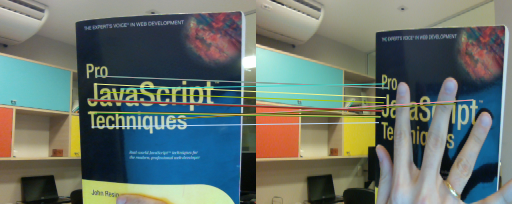
\includegraphics[width=\linewidth]{chapters/evaluation/keypoints_occlusion.png}
  \caption{Library implementation of markerless tracking technique partial occlusion robustness.}
  \label{figure:keypoints_occlusion}
\end{figure}

% subsubsection occlusion_robustness (end)

% subsection results (end)

\subsection{Discussion} % (fold)
\label{sub:evaluation:markerless_tracking_algorithm:discussion}

Tracking based on natural features characteristics is promising since it doesn't require any artificial marker in order to facilitate tracking. Future work is required in order to leverage this technique to be robust enough in order to be used in real large applications. The first improvement is to improve overall performance of the feature detection phase. For feature detection FAST-ER can be used in replacement of the existing FAST detector in order to improve repeatability, resulting in better performance \cite{RostenFaster2010}. On the results subsection \ref{sub:evaluation:markerless_tracking_algorithm:results}, this technique implementation on the web has presented average of 6 FPS, which is below the PAL threshold of real-time rate. The second improvement is to provide a Perspective-$n$-Point problem (P$n$P) calculation. The aim of the P$n$P is to determine the position and orientation of a camera given its intrinsic parameters and a set of $n$ correspondences between 3D points and their 2D projections. It has many applications in Computer Vision, Robotics, AR and Computer Vision \cite{Hartley2004} communities. One strong candidate algorithm is called EP$n$P proposed by Lepetit et al. on \cite{Lepetit2008}, as a non-iterative solution to the P$n$P problem, which is the estimation of the pose of a calibrated camera from $n$ 3D-to-2D point correspondences, whose computational complexity grows linearly with $n$. This is in contrast to state-of-the-art methods that are $O(n^5)$ or even $O(n^8)$. Lepetit's method handles properly both planar and non-planar configurations and also have low computational complexity \cite{Lepetit2008}.

% subsection discussion (end)

% section markerless_tracking_algorithm (end)

\section{Benefits of a JavaScript tracking solution} % (fold)
\label{sec:evaluation:js_tracking_solution}

\subsubsection{Discussion} % (fold)
\label{subsub:evaluation:results:js_tracking_solution:description}

On Markerless Tracking Solutions for Augmented Reality on the Web \cite{Pablo2013}, a server-side tracking solution was implemented and the developed solution showed to be not scalable, causing a delay in the exhibition of the AR result when having more than five simultaneous users. This way, the adopted distributed approach turned out to be not adequate to web targeted applications, where hundreds of simultaneous users should be capable of using it. In the same work \cite{Pablo2013}, Pablo et al., proposed a client-side solution that requires a third-party plugin installation called OSAKit \cite{OSAKit2013}. The OSAKit plugin allows desktop applications to run without loss of performance inside most current browsers on the Windows platform. The results were promising in terms of FPS reached (25 FPS), although the average load time of the application was $11$ minutes (due to the size of the precomputed data, $22$ MB), considering a broadband connection of $256$ Kbps. Using a pure JavaScript tracking solution has shown to be very effective since the FPS average is the same with a smaller size. On Table \ref{table:comparison_with_osakit}, a comparison between the size, loading time and FPS between the OSAKit solution and \textit{tracking.js} is presented.

\begin{table}[!htb]
    \centering % here
    \begin{tabular}{|c|c|c|c|}
        \hline
        & OSAKit & \textit{tracking.js} + color & \textit{tracking.js} + face \\
        \hline
        Average frame rate & 25 FPS & 30 FPS & 25 FPS\\
        \hline
        Average file size & 22 MB & 8 KB & 187 KB\\
        \hline
        Average load time (256 Kbps) & 11 min & 0.25 seconds & 5 seconds\\
        \hline
    \end{tabular}
    \caption{Comparison between \textit{tracking.js} and OSAKit client-side tracking solution.}
    \label{table:comparison_with_osakit}
\end{table}

% subsection description (end)

% section js_tracking_solution (end)

% chapter evaluation (end)